% !TeX program = xelatex
% !TeX encoding = UTF-8
\documentclass[aspectratio=169]{beamer}

% ----------------- Theme -----------------
\usetheme{Madrid}
\usecolortheme{default}
\setbeamertemplate{navigation symbols}{}
\setbeamersize{text margin left=0.7cm, text margin right=0.7cm}

% ----------------- Packages -----------------
% Compile with xelatex or lualatex for Chinese\n\usepackage{ctex}
\usepackage{graphicx}
\usepackage{booktabs}
\usepackage{amsmath, amssymb}
\usepackage{tikz}
\usetikzlibrary{arrows.meta, positioning}
\usepackage{adjustbox}
\usepackage[UTF8]{ctex}
\graphicspath{{./}}

% ----------------- Image helpers -----------------
\newcommand{\fitimg}[1]{%
  \begin{center}
    \adjustbox{max size={\textwidth}{0.78\textheight}}{\includegraphics{#1}}
  \end{center}
}

% Split a tall figure into top/bottom parts by relative height (no overlap)
% #1 = fraction to trim (e.g., 0.52), #2 = filename
\newcommand{\fitimgTopPart}[2]{%
  \begin{center}
    \adjustbox{max size={\textwidth}{0.80\textheight}}{%
      \adjustbox{trim=0 {#1\height} 0 0,clip}{\includegraphics{#2}}%
    }
  \end{center}
}
\newcommand{\fitimgBottomPart}[2]{%
  \begin{center}
    \adjustbox{max size={\textwidth}{0.80\textheight}}{%
      \adjustbox{trim=0 0 0 {#1\height},clip}{\includegraphics{#2}}%
    }
  \end{center}
}

% ----------------- Title Info -----------------
\title[Project B]{Employment \& Unemployment Insights from Search Data}
\subtitle{Baidu Index + Baidu Baike: Acquisition, Index Construction, Descriptive Analysis}
\author{Chenxi Zhang \and Haowen Shi \and Haotian Zhou}
\institute{Data Science \& AI Course Project (Project B)}
\date{December 25, 2025}

\begin{document}

% =========================================================
\begin{frame}
  \titlepage
\end{frame}

% =========================================================
\begin{frame}{Outline}
\begin{enumerate}
  \item Background \& Objectives
  \item Midterm Plan (Scope, Deliverables, Roles)
  \item Data Sources \& Acquisition
  \item Cleaning \& Preprocessing
  \item Index Construction (Sub-indices \& Composite)
  \item Results \& Visualization
  \item Robustness \& Discussion
  \item Conclusion \& Next Steps
\end{enumerate}
\end{frame}

% =========================================================
\section{Background and Objectives}

\begin{frame}{Background}
\begin{itemize}
  \item Employment/unemployment is closely tied to social stability and macro conditions.
  \item Search interest provides a high-frequency \textbf{proxy} for public concern and job-market sentiment.
  \item We combine \textbf{Baidu Index} (behavioral signal) with \textbf{Baidu Baike} (concept/policy context) for interpretability.
\end{itemize}

\begin{block}{Project Objective}
Construct an interpretable \textbf{labor-market attention index} and summarize descriptive findings (trend, distribution, robustness).
\end{block}
\end{frame}

\begin{frame}{Research Questions}
\begin{enumerate}
  \item How does search interest in employment/unemployment topics evolve over time?
  \item Can multiple keywords be aggregated into meaningful \textbf{sub-indices} and a \textbf{composite index}?
  \item Are the main patterns stable under different normalization and aggregation choices?
\end{enumerate}
\end{frame}

% =========================================================
\section{Midterm Plan Elements}

\begin{frame}{Midterm Plan: Scope \& Deliverables}
\begin{block}{Scope (planned)}
China, past five years (2019--2025).
\end{block}

\begin{block}{Deliverables (planned)}
Clean datasets, descriptive analytics, and clear visuals; reproducible code + report/slides.
\end{block}

\begin{block}{Pipeline (planned)}
\begin{itemize}
  \item Data Collection (Baidu Index \& Baidu Baike)
  \item Data Cleaning (missingness/duplicates/outliers)
  \item Descriptive Analysis (distribution/correlation/trends)
  \item Visualization (time trends, comparisons)
  \item Conclusions \& Outlook
\end{itemize}
\end{block}
\end{frame}

\begin{frame}{Midterm Plan: Timeline \& Team Roles}
\begin{columns}[T,onlytextwidth]
\column{0.55\textwidth}
\begin{block}{Timeline (next 4--5 weeks)}
\begin{itemize}
  \item Week 1: finalize keyword list; collect Index \& Baike; build raw database
  \item Week 2: cleaning pipeline; missing/outlier handling; unify region codes
  \item Week 3: descriptive analysis; correlation/trends; event annotations
  \item Week 4: visualization polishing; interpret results; draft report/slides
  \item Week 5 (optional): forecasting / policy comparison
\end{itemize}
\end{block}

\column{0.45\textwidth}
\begin{block}{Roles \& Allocation}
\begin{itemize}
  \item Chenxi Zhang: keyword design; Index export; regional comparison
  \item Haowen Shi: Baike text structuring; text mining/topic sketches
  \item Haotian Zhou: cleaning scripts; time-series plots; robustness checks
\end{itemize}
\end{block}
\end{columns}
\end{frame}

% =========================================================
\section{Data Sources and Acquisition}

\begin{frame}{Data Sources}
\begin{block}{Baidu Index (Primary quantitative source)}
Keyword-level search index time series (configurable by time window and region).
\end{block}

\begin{block}{Baidu Baike (Contextual source)}
Definitions / categories / policy background used to justify keyword selection and grouping.
\end{block}

\begin{block}{Current dataset used in this report}
Monthly series from 2023-01 to 2024-12 (24 timestamps), 42 keywords across 4 sub-domains.\\
Note: overlapping keywords (e.g., 临时工、兼职、蓝领招聘) appear in multiple sub-domains by design.
\end{block}
\end{frame}

\begin{frame}{Data Acquisition}
\begin{block}{Baidu Index collection}
\begin{itemize}
  \item Define keyword list and sub-domain mapping.
  \item Export index series for a chosen time window (and region if needed).
  \item Store into structured tables for downstream processing.
\end{itemize}
\end{block}

\begin{block}{Baidu Baike collection}
\begin{itemize}
  \item Scrape targeted entries (policies, unemployment types, etc.).
  \item Extract structured text fields to support interpretability and later text mining.
\end{itemize}
\end{block}
\end{frame}

% =========================================================
\section{Cleaning and Preprocessing}

\begin{frame}{Data Cleaning}
\begin{itemize}
  \item \textbf{Completeness}: check missing timestamps/keywords; interpolate or drop with records.
  \item \textbf{Duplicates}: ensure uniqueness within each (Timestamp, Keyword, Domain) key.
  \item \textbf{Outliers}: flag abnormal spikes (3$\sigma$/IQR); keep if event-driven.
  \item \textbf{Formatting}: unify date formats and numeric types; consistent encoding.
\end{itemize}
\end{frame}

\begin{frame}{Normalization}
\begin{block}{Why normalize?}
Keyword series have different scales; normalization prevents dominance by large-scale keywords.
\end{block}

\begin{block}{Two baseline methods}
\[
\text{MinMax: } x'=\frac{x-\min(x)}{\max(x)-\min(x)}
\qquad\qquad
\text{Z-score: } x'=\frac{x-\mu}{\sigma}
\]
\end{block}
\end{frame}

% =========================================================
\section{Index Construction}

\begin{frame}{Sub-domains \& Keyword Design (Updated)}
\begin{block}{Four sub-domains (updated after instructor feedback)}
\begin{enumerate}
  \item 求职活跃度 (Job-search \& Hiring Demand)
  \item 就业困难/就业压力 (Employment Difficulty / Uncertainty)
  \item 失业/裁员/再就业压力 (Unemployment \& Layoff Pressure)
  \item 结构性/弱势群体就业压力 (Structural / Precarious Employment Stress)
\end{enumerate}
\end{block}

\begin{block}{Notes on overlapping keywords}
Some terms (e.g., “兼职/临时工/蓝领招聘”) can reflect both general labor demand and structural stress.
We keep the mapping explicit and use robustness checks to test alternative assignments.
\end{block}
\end{frame}

\begin{frame}{Keyword List (Final)}
\footnotesize
\begin{columns}[T,onlytextwidth]
\column{0.5\textwidth}
\textbf{求职活跃度}:找工作,招聘,求职,招聘信息,校招,春招,秋招,面试,简历

\vspace{0.6em}
\textbf{就业困难/压力}:就业难,找工作难,应届生就业,应届生找工作,就业形势,就业前景,行业前景,薪资水平,薪资查询,大学生就业,毕业生就业

\column{0.5\textwidth}
\textbf{失业/裁员压力}:失业,裁员,裁员潮,被裁,优化,失业金,失业保险,失业补助,失业登记,再就业,低门槛工作,临时工,兼职,蓝领招聘

\vspace{0.6em}
\textbf{结构性/弱势群体压力}:35岁就业,35岁找工作,中年就业,蓝领招聘,低学历就业,外卖骑手,快递员,送外卖,兼职,临时工,底层劳动岗位
\end{columns}
\end{frame}

\begin{frame}{Sub-indices and Composite Index}
\begin{block}{Sub-index (group average)}
For sub-domain $d$ with keyword set $\mathcal{K}_d$:
\[
S_d(t)=\frac{1}{|\mathcal{K}_d|}\sum_{k\in \mathcal{K}_d} x'_k(t)
\]
\end{block}

\begin{block}{Composite index (baseline)}
\[
I(t)=\sum_{d=1}^{4} w_d\,S_d(t),\qquad \sum_{d=1}^{4} w_d=1
\]
Baseline: equal weights. Robustness: Z-score normalization / MPI aggregation / alternative weights.
\end{block}
\end{frame}

\begin{frame}{Current Sub-index Snapshot (t = 2023-01)}
\small
\begin{table}
\centering
\begin{tabular}{lcc}
\toprule
Sub-domain & Interpretation & Value \\
\midrule
求职活跃度 & job-search intensity & 6.88 \\
就业困难/压力 & perceived difficulty/uncertainty & 18.76 \\
失业/裁员压力 & unemployment/layoff concern & 70.63 \\
结构性/弱势群体压力 & structural/precarious stress & 62.87 \\
\bottomrule
\end{tabular}
\end{table}
\end{frame}

\begin{frame}{Processing Pipeline}
\centering
\adjustbox{max size={\textwidth}{0.55\textheight}}{%
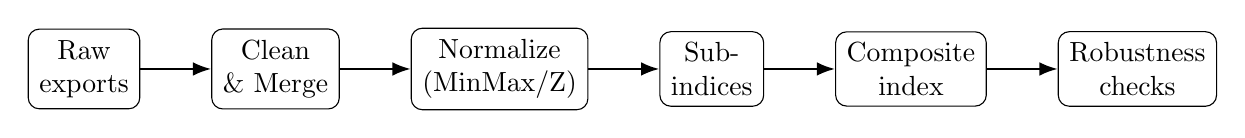
\begin{tikzpicture}[
  box/.style={draw, rounded corners, align=center, inner sep=4pt},
  arr/.style={-Latex, thick},
  node distance=0.75cm and 0.9cm
]
\node[box] (raw) {Raw\\exports};
\node[box, right=of raw] (clean) {Clean\\\& Merge};
\node[box, right=of clean] (norm) {Normalize\\(MinMax/Z)};
\node[box, right=of norm] (sub) {Sub-\\indices};
\node[box, right=of sub] (comp) {Composite\\index};
\node[box, right=of comp] (rob) {Robustness\\checks};

\draw[arr] (raw) -- (clean);
\draw[arr] (clean) -- (norm);
\draw[arr] (norm) -- (sub);
\draw[arr] (sub) -- (comp);
\draw[arr] (comp) -- (rob);
\end{tikzpicture}
}
\vspace{0.5em}
\small Reproducible workflow implemented in the repository scripts and exported tables.
\end{frame}

% =========================================================
\section{Results and Visualization}

\begin{frame}{Descriptive Summary (Composite Index)}
\begin{block}{Basic statistics (2023-01 to 2024-12)}
\begin{itemize}
  \item Mean: 36.57 \qquad Std: 19.47
  \item Min: 6.12 \qquad Max: 71.53
  \item Outliers (3$\sigma$ rule): none detected
\end{itemize}
\end{block}

\begin{block}{Peak / trough months (examples)}
\begin{itemize}
  \item Top-3 peaks: 2024-12 (71.53);2024-07 (65.83);2024-06 (65.61)
  \item Bottom-3 troughs: 2023-02 (6.12);2023-05 (6.63);2023-04 (10.90)
\end{itemize}
\end{block}
\end{frame}

\begin{frame}[t]{Result Figure: Labor Market Index Analysis}
\vspace{-0.6em}
\fitimg{labor_market_index_analysis.png}
\vspace{-0.8em}
\end{frame}

\begin{frame}[t]{Result Figure: Report Snapshot (Top)}
\vspace{-0.6em}
% Same split ratio -> small gap -> no overlap
\fitimgTopPart{0.42}{labor_market_analysis_report.png}
\end{frame}

\begin{frame}[t]{Result Figure: Report Snapshot (Bottom)}
\vspace{-0.6em}
\fitimgBottomPart{0.58}{labor_market_analysis_report.png}
\end{frame}

% =========================================================
\section{Robustness and Discussion}

\begin{frame}{Robustness Check (Alternative Constructions)}
\begin{block}{What we compare}
\begin{itemize}
  \item Base Case vs Z-score normalization
  \item Linear aggregation vs MPI (non-compensatory aggregation)
  \item Equal weights vs alternative weights
\end{itemize}
\end{block}

\begin{block}{Correlation (higher means more consistent)}
\small
\begin{table}
\centering
\begin{tabular}{lcccc}
\toprule
 & Base & ZScore & MPI & Weights \\
\midrule
Base    & 1.000000 & 0.999942 & 0.939957 & 0.982355 \\
ZScore  & 0.999942 & 1.000000 & 0.939331 & 0.982513 \\
MPI     & 0.939957 & 0.939331 & 1.000000 & 0.917450 \\
Weights & 0.982355 & 0.982513 & 0.917450 & 1.000000 \\
\bottomrule
\end{tabular}
\end{table}
\end{block}
\end{frame}

\begin{frame}{Limitations}
\begin{itemize}
  \item Search attention is a \textbf{proxy}, not official unemployment/employment measurement.
  \item News/viral events may create temporary spikes unrelated to structural changes.
  \item Keyword choice and mapping may introduce subjectivity $\rightarrow$ sensitivity analysis is necessary.
\end{itemize}
\end{frame}

% =========================================================
\section{Conclusion}

\begin{frame}{Conclusion \& Next Steps}
\begin{block}{Conclusion}
\begin{itemize}
  \item Built a reproducible pipeline from Baidu Index keyword series to 4 sub-indices and a composite index.
  \item Produced descriptive summaries and visualizations of labor-market attention dynamics.
  \item Verified stability under multiple construction choices (normalization/aggregation/weights).
\end{itemize}
\end{block}

\begin{block}{Next Steps (from plan)}
Extend to full 2019--2025 window; enrich Baike text mining (TF-IDF/topic sketches); add event and regional comparisons; optional external validation with official statistics.
\end{block}
\end{frame}

\begin{frame}[plain]
\vfill
\centering
{\Huge Q \& A}
\vfill
\end{frame}

\end{document}
